\section{Problem4: Validation and Expansion of MM-LSTM }

%%%%%%%%%%%%%%%
%% TODO
%%%%%%%%%%%%%%%
\subsection{Prediction of Momentum Swings}

Based on the MM-LSTM model established earlier, we used a match as the test set and obtained the corresponding output results:

\begin{figure}[htbp]
    \centering
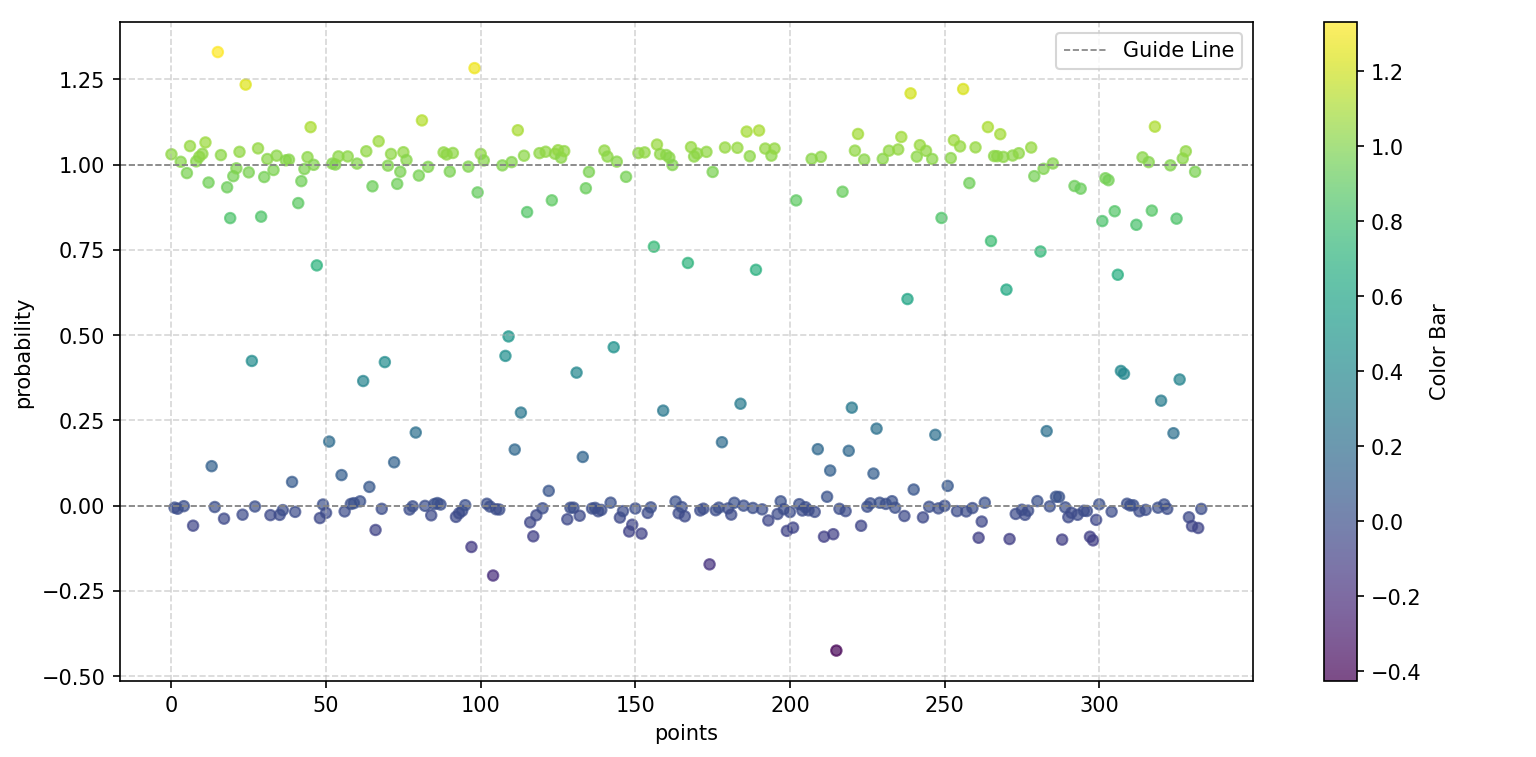
\includegraphics[width=1\textwidth]{figure/prediction_value_distribution.png}
    % \vspace{-0.3cm}
    \caption{Scatter Plot of Probability Values Predicted Using MM-LSTM Model}
    % \label{fig:gradients_pie}
    % \vspace{-0.5cm}
\end{figure}

We will calculate the probability value using the Equation \ref{eq:formula26}  and Equation \ref{eq:formula27} obtained from 5.1 to obtain $\eta_{\text{accuracy}} = 90.71\%$, the fitting effect is good. We will use Equation \ref{eq:formula25} to calculate the predicted relative slope curve of the fitted data, and plot the curve with the real data in the following figure:



\begin{figure}[htbp]
    \centering
     \hspace*{-1.2cm} % 负值表示左移
    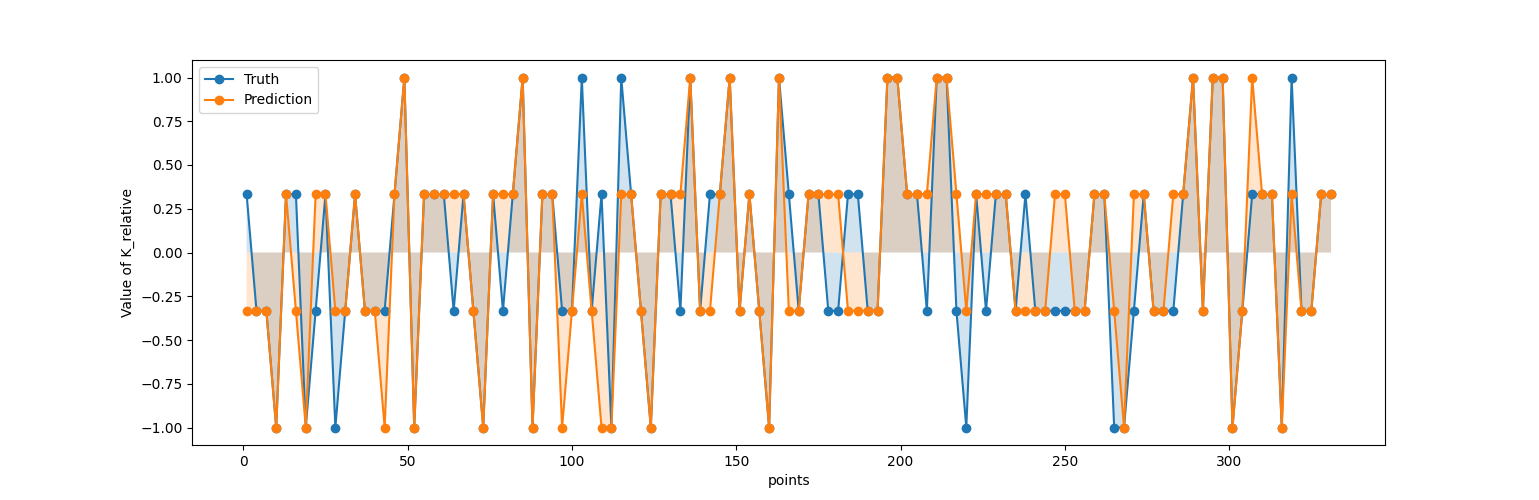
\includegraphics[width=1.1\textwidth]{figure/Figure_1.png}
    % \vspace{-0.3cm}
    \caption{The Fitting Effect of Momentum True Value and Predicted Value}
    % \label{fig:gradients_pie}
    % \vspace{-0.5cm}
\end{figure}

% 在以上图中我们可以得出,预测的动量波动曲线大部分均与真实动量波动曲线重叠,经测算拟合的决定系数R^{2}=61.51%,相关性与预测准确率相差较大可能是由于拟合系数与预测值是斜率和函数值的关系以及选取的时间段并不是一小部分而是一段时间导致的,在计算中当时间段points个数为3的时候拟合效果最好,我们认为过短导致图像波动过大拟合效果差,过长导致起伏都被均值化,无法体现出来。

In the above figures, we can observe that the predicted momentum fluctuation curve largely overlaps with the actual momentum fluctuation curve. The calculated coefficient of determination \(R^2\) is \(61.51\%\), indicating a moderate level of fit. The discrepancy between correlation and prediction accuracy could be attributed to the relationship between the fitting coefficient and predicted values, which involves the slope and function values. Additionally, the chosen time period is not a small subset but rather a segment, contributing to the observed difference. In the calculations, the best fitting performance is achieved when the number of data points in the time period is 3. We believe that too short a time span leads to excessive fluctuation in the graph, resulting in poor fitting performance. On the other hand, an overly long time span tends to average out the swings, making it challenging to capture the nuances.



\subsection{Future Model Influence Factors Analysis}
Based on the analysis of the above model prediction results, although it has reached 90.71\% belonging to the acceptable range of the predictive model; however, the model influence factor mainly focuses on the athletes' performance in the competition and its quantitative indexes, and it does not take into account many factors other than non-athletic performance factors. Therefore the assessment and quantification of subjective and objective factors of non-athletic performance is a direction that can be further optimized in the future model.

\subsubsection{Objective Factors}
The above model mainly analyzes the data of Wimbledon, where "serve is king", so the proportion of serve-related factors in the prediction model is high. However, in addition to Wimbledon, there are also the Australian Open, the US Open and the French Open among the four major tennis tournaments. Each tournament has its own unique characteristics, especially the venue factor is particularly prominent, such as Table \ref{tab:tennis_courts} is the analysis of the characteristics of different venues.

\begin{table}[htbp]
    \centering
    \caption{Tennis Court Characteristics and Associated Tournaments} 
    \vspace{8pt}
    \label{tab:tennis_courts}
    \begin{tabular}{c|cccc}
        \toprule[1.5pt]
        Court Type & Ball Speed & Return Height & Return Speed & Delegate Competition\\
        \midrule[1pt]
        Clay Courts & 1 & Very High & Medium & French Open \\
        Hard Courts & 2 & Stable & Fast & Australian Open \& U.S. Open \\
        Grass Courts & 4 & High & Very Fast & Wimbledon Championships \\
        Carpet Courts & 3 & Medium & Medium & ATP Indoor Race \\
        \bottomrule[1.5pt]
    \end{tabular}
\end{table}


Non-standardized court surface criteria are detrimental to the generality of the prediction model; the strong correlation between serve and rally speeds on grass at Wimbledon led players to generally adopt aggressive attacking strategies and serve to win; conversely, French Open players were more conservative, resulting in the longest average court time of the French Open matches. To enhance the predictive model, the training set can be extended to various court conditions. Ultimately, including court conditions as an influencing factor will improve the overall predictive accuracy of future models.

\subsubsection{Subjective Factors}
The subjective factors of the game are difficult to quantify, in which the psychological quality and the strength of the comparison is mutual influence, affecting the trend of the game. The level of the opponent indirectly affects the psychological state of the player, when encountering stronger opponents, may be nervous, resulting in malfunctioning; or there will be a "strong is strong" phenomenon can be over-performed. Correspondingly, when encountering weaker opponents, different psychological fluctuations will also occur, but the degree to which the psychological fluctuations affect the performance of different players varies. Therefore, it is very important for players to develop their self-regulation ability, anti-stress ability, and the ability to adapt to the venue from the experience of the tournament.

\subsection{Testing the generalizability of the model on table tennis matches}
To test the generalizability of our model across other sports, we collected data from the WTT 2024 table tennis matches. We trained and tested the model on a dataset consisting of 1515 table tennis matches. We partitioned 80\% of the data for training and reserved the remaining 20\% for testing. After training for 1000 epochs, our model achieved a prediction accuracy of 75.574\% on the test set, which did not reach the prediction accuracy achieved in tennis.


To analyze the reasons for the unsatisfactory performance of the model, we compared the collected data from the WTT 2024 matches with the data provided by MCM on the Wimbledon 2023 Gentlemen’s singles matches after the second round. We believe that the suboptimal prediction results in table tennis matches are due to the following two factors:

\begin{enumerate}
    \item The quantity of data collected for table tennis matches is relatively small. The tennis dataset comprises 7,285 data entries, whereas the table tennis dataset contains only 1,515 data entries, amounting to just 20.8\% of the tennis data in terms of entry count.
    \item The table tennis dataset lacks a variety of metrics compared to the tennis dataset. The table tennis data includes only the match ID, player names, and the scores of each player, without various in-game state metrics (such as "p1\_double\_fault" and "p2\_double\_fault"). Consequently, the total count of metrics in the table tennis data sums up to 6,060. In contrast, the tennis data, when counted by the number of metrics, totals 335,110. In summary, the sum of the table tennis metrics accounts for only 1.8\% of the total count of metrics in the tennis dataset.

\end{enumerate}

In conclusion, we believe that the MM-LSTM model we designed exhibits a certain degree of generality. However, its performance is constrained by the limited quantity of data. If more match data can be collected to allow the model to learn a greater variety of match-related information, there is substantial potential for improvement in model performance.
